\documentclass[../../main.tex]{subfiles}

\graphicspath{{../../image/}{../../figure/}}

\begin{document}

\section{图像分割}\label{section:ch10-图像分割}

在图像分类问题中，整个图像被分配了单一类别标签。我们已经看到，如果检测多个对象并使用边界框记录它们的位置，则可以提供更详细的信息（参见10.4节）。语义分割（semantic segmentation）可以让我们获得更详细的分析，其中图像的每个像素被分配给预设的类别之一。这意味着输出空间的维度与输入图像的维度相同，因此可以方便地表示为具有相同像素数量的图像。尽管输入图像通常具有R、G、B三个通道，但输出数组具有$C$个通道（假设有$C$个类别）以表示每个类别的概率。如果我们将每个类别与不同的（任意选择的）颜色关联起来，那么分割网络的预测可以表示为一幅图像，其中每个像素根据具有最高概率的类别着色，如图10.26所示。

\subsection{卷积分割}\label{subsection:ch10-卷积分割}

一种解决语义分割问题的简单方法是构建一个卷积网络，该网络将图像上以某个像素为中心的矩形部分作为输入，并借助单一softmax输出对该像素进行分类。通过将这样的网络轮流应用于每个像素，便可以分割整个图像（这需要根据输入窗口的大小在图像周围进行边缘填充）。然而重叠部分会导致冗余计算，使得这种方法十分低效（参见图10.21）。我们可以通过将不同输入位置的前向传播计算组合输入单一网络来消除这种低效性，得到一个最终的全连接层也是卷积层的模型（参见图10.23）。因此，我们可以构建一个在每层都使用步幅为1、做了等大填充且没有池化的CNN，从而使得每一层的维度都与输入图像的维度相同。每个输出单元都具有softmax激活函数，权重在所有输出之间共享。虽然可能有效，但这样的网络仍然需要许多层，且每层中有多个通道，以学习实现高精度所需的复杂内部表示。如果这样做，即使对于常规分辨率的图像，计算成本也是难以承受的。

\subsection{上采样}\label{subsection:ch10-上采样}

大多数卷积网络使用多层下采样，从而在通道数量增加的同时，使特征图的大小减小，以及在确保网络整体大小和计算成本可控的同时，允许网络从图像中提取高阶语义特征。我们可以利用这个概念来创建一个更高效的语义分割架构。该架构采用标准的深度卷积网络，并添加了一些额外的可学习层，这些额外的可学习层用于将低维的内部表示转换回原始图像分辨率（Long, Shelhamer, and Darrell, 2014; Noh, Hong, and Han, 2015; Badrinarayanan, Kendall, and Cipolla, 2015），如图10.27所示。

为了做到这一点，我们需要一种方法来逆转跨步卷积和池化操作的下采样效果。首先考虑类比于池化的上采样操作，其中输出层的单元数比输入层的单元数多，例如每个输入单元对应一个$2\times 2$的输出单元块。接下来的问题是输出应该使用什么值。为了找到类比于平均池化的上采样操作，我们可以简单地将每个输入值复制到所有对应输出单元中，如图10.28(a)所示。可以看到，对这个操作的输出应用平均池化即可重新生成输入。

对于最大池化，我们可以考虑图10.28(b)中的操作，其中将每个输入值复制到相应输出块的第一个单元中，并将每个输出块中的其余值置零。同样，我们看到对输出层应用最大池化操作会重新得到输入层。这有时称为最大上采样（max-unpooling）。将非零值分配给输出块的第一个单元似乎是任意的，因此可以使用一种保留了更多来自下采样层的空间信息的改进方法（Badrinarayanan, Kendall, and Cipolla, 2015）。这是通过设计一种网络架构来实现的，该架构在每个最大池化下采样层之后都有一个相应的上采样层。在下采样过程中，记录每个输出块中的哪个单元具有最大值，接着在相应的上采样层中，将非零元素设置到相同的位置，如图10.29中的$2\times 2$最大池化所示。

前面讨论的上采样操作都是固定的函数，类似于平均池化和最大池化的下采样操作。我们也可以使用一种称为学习到的（learned）上采样操作，类比于用于下采样的跨步卷积。在跨步卷积中，输出图上的每个单元通过共享可学习权重与输入图上的一小块相连。当我们在输出数组中移动一步时，滤波器在输入数组上将移动两步或更多步，因此输出数组的维度小于输入数组的维度。对于上采样，我们使用一个滤波器将输入数组中的一个像素连接到输出数组中的一小块。然后选择架构，使得当在输入数组中移动一步时，在输出数组中移动两步或更多步（Dumoulin and Visin, 2016）。图10.30说明了应用$3\times 3$滤波器和输出步幅为2的情况。注意，存在多个滤波器位置重合的输出单元，在这种情况下，相应的输出值可以通过对来自各个滤波器位置的贡献进行求和或求平均来计算。这种上采样称为转置卷积（transpose convolution），因为如果将下采样卷积表示为矩阵形式，则相应的上采样卷积可以由转置矩阵给出（见习题10.13）。注意，有时也称这种上采样为“反卷积”，但最好避免使用这个术语，因为在数学中“反卷积”通常表示泛函分析中卷积的逆操作，概念完全不同。转置卷积又称“分数跨步卷积”，因为标准卷积的步幅是输出层步长与输入层步长的比值。

\subsection{全卷积网络}\label{subsection:ch10-全卷积网络}

如果我们的网络架构没有池化层，即下采样和上采样纯粹使用卷积来完成，则称这样的网络为全卷积网络（fully convolutional network）（Long, Shelhamer, and Darrell, 2014）。全卷积网络可以接收任意大小的图像，并输出相同大小的分割图。这可以看作$3\times 3$卷积的逆运算。

\subsection{U-Net架构}\label{subsection:ch10-U-Net架构}

我们已经看到，与跨步卷积和池化相关的下采样允许增加通道的数量，而不会使网络的规模变得过大。但这也会降低空间分辨率，导致信号流过网络时丢失位置信息。虽然这对于图像分类来说是可以接受的，但对于图像语义分割来说，丢失空间信息是一个大问题，因为我们想要分类每个像素。解决这个问题的一种方法是使用U-Net架构（Ronneberger, Fischer, and Brox, 2015），如图10.31所示，其名称来自示意图所示的U形结构。其核心概念是，对于每个下采样层，都有一个对应的上采样层，并且每个下采样层的输出被拼接到相应的上采样层，从而使这些上采样层能够获得更高分辨率的空间信息。注意，可以在U-Net架构的最后一层使用$1\times 1$卷积将通道数量减少至类别数量，然后接一个softmax激活函数。

\begin{figure}[htbp]
  \centering
  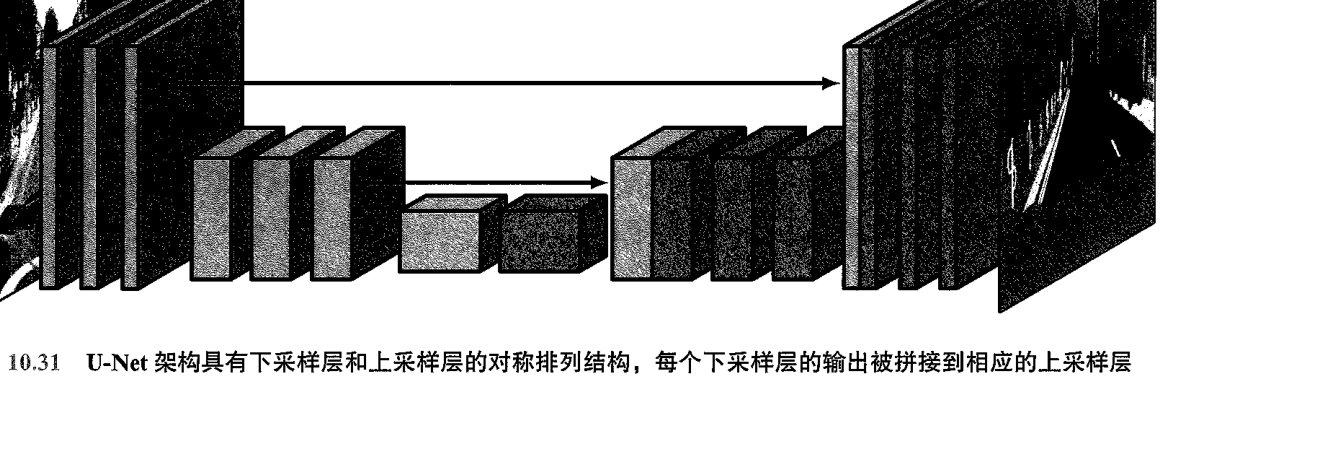
\includegraphics[width=0.85\textwidth]{ch10-fig303-unet.png}
  \caption{U-Net架构具有下采样层和上采样层的对称排列结构，每个下采样层的输出被拼接到相应的上采样层。}
  \label{figure:ch10-U-Net架构}
\end{figure}

\end{document}
